\begin{figure}[htbp]
  \centering
  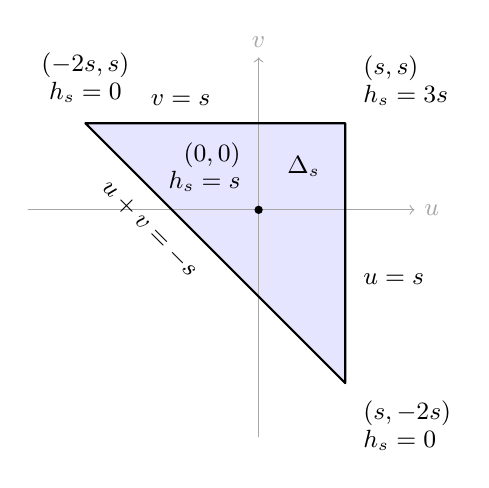
\begin{tikzpicture}[x=1.10cm,y=1.10cm,line cap=round,line join=round,
                      font=\small]
    \fill[blue!10] (-2,1) -- (1,1) -- (1,-2) -- cycle;
    \draw[gray!70,->] (-2.66,0) -- (1.80,0) node[right] {$u$};
    \draw[gray!70,->] (0,-2.62) -- (0,1.76) node[above] {$v$};
    \draw[thick] (-2,1) -- (1,1) -- (1,-2) -- cycle;
    \node[above=4pt,align=center] at (-2,1)
      {$(-2s,s)$\\[-1pt] $h_s=0$};
    \node[above right=3pt,align=left] at (1,1)
      {$(s,s)$\\[-1pt] $h_s=3s$};
    \node[below right=3pt,align=left] at (1,-2)
      {$(s,-2s)$\\[-1pt] $h_s=0$};
    \node[above=3pt] at (-.90,1) {$v=s$};
    \node[right=3pt] at (1,-.80) {$u=s$};
    \node[rotate=-45,below=4pt] at (-1.02,.02) {$u+v=-s$};
    \node at (.52,.50) {$\Delta_s$};
    \fill (0,0) circle[radius=1.5pt];
    \node[above left=3pt,align=right] at (0,0)
      {$(0,0)$\\[-1pt] $h_s=s$};
  \end{tikzpicture}
  \[
    \int_{\Delta_s}h_s(u,v)\,du\,dv
    =\underbrace{\frac{(3s)^2}{2}}_{\text{area}}
      \underbrace{\frac{3s+0+0}{3}}_{\text{mean affine height}}
    =\frac{27s^3}{6}.
  \]
  \caption{For fixed $T=s>0$, the positive integrand is supported,
  within $u\le s$ and $v\le s$, on
  $\Delta_s=\{(u,v):u\le s,\ v\le s,\ s+u+v\ge0\}$.
  Here $h_s(u,v)=s+u+v$ is an affine height, with the displayed values at
  the vertices and barycenter. The shading marks the integration region,
  not the support or density of the Gaussian pair $(U,V)$.
  Multiplying the unweighted integral by the density bound $M$ gives
  the estimate used in the proof. At $s=0$ the triangle degenerates and
  the integral is zero.}
  \label{fig:residual-score-triangle}
\end{figure}
